The maximum required  output  power  of  our  device  was  roughly  calulated as
$\SI{24}{\volt} \cdot \SI{3}{\ampere} = \SI{72}{\watt}$.  Assuming an efficiency
of $\eta\approx \SI{90}{\percent}$ an \SI{80}{W} power supply is required.

The design and construction of a  custom  power  supply  would have consumed too
much  time and resources. Instead, we opted for an external power  supply  which
can be mounted inside the  housing.  The  selected  power  supply  is capable of
supplying  \SI{28}{\volt}  at   \SI{75}{\watt}   and   can  be  seen  in  figure
\ref{fig:circuit:mains-input}.

\begin{figure}[th!]
    \centering
    \begin{minipage}{.3\textwidth}
        \centering
        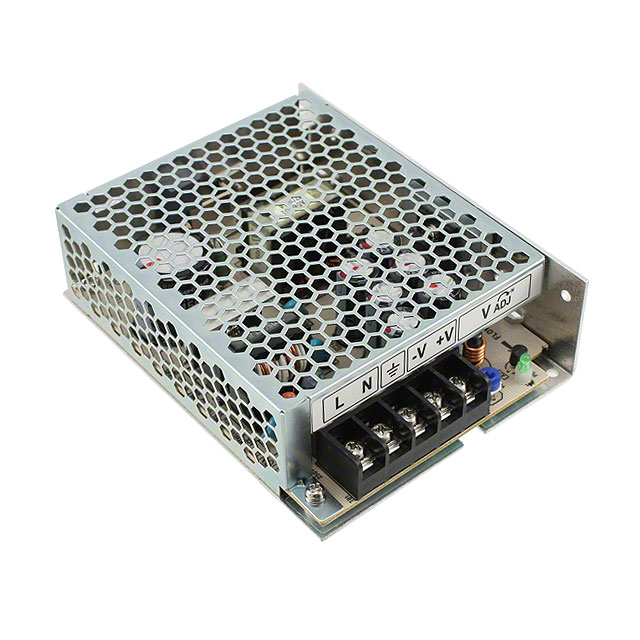
\includegraphics[width=\textwidth]{images/circuit/external-power-supply.JPG}
        \caption{External PSU}
        \label{fig:circuit:mains-input}
    \end{minipage}
    \begin{minipage}{.3\textwidth}
        \centering
        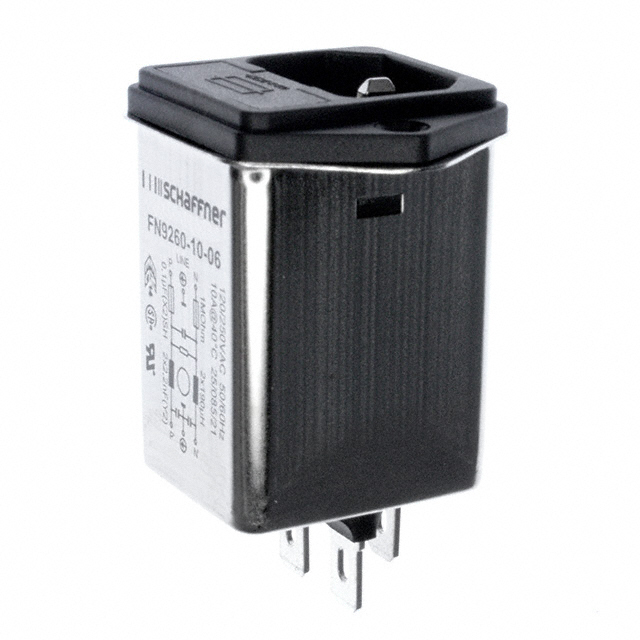
\includegraphics[width=.9\textwidth]{images/circuit/power-entry-module.JPG}
        \caption{Power Entry Module}
        \label{fig:circuit:iec60320c13}
    \end{minipage}
    \begin{minipage}{.3\textwidth}
        \centering
        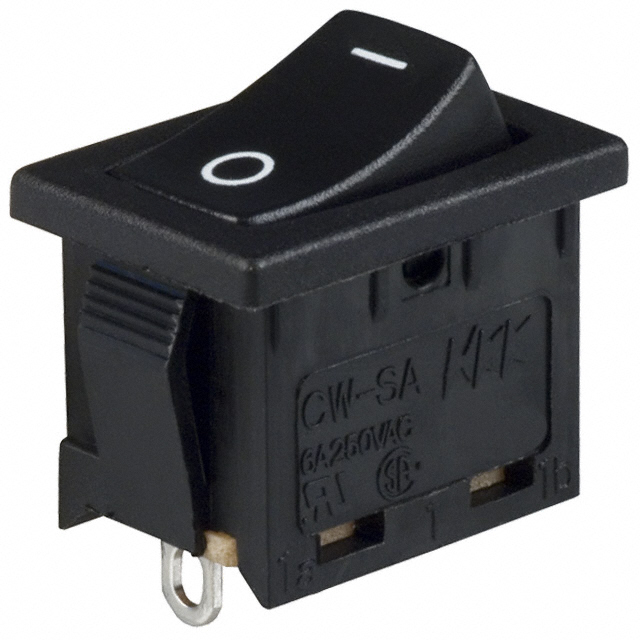
\includegraphics[width=.6\textwidth]{images/circuit/rocker-switch.JPG}
        \caption{Rocker Switch}
        \label{fig:circuit:rocker-switch}
    \end{minipage}
\end{figure}

The  device  can be plugged into a power outlet by means of  an  IEC  60320  C13
socket seen in figure \ref{fig:circuit:iec60320c13}. The socket has a
built-in  fuse  as  well  as  a  built-in  mains  filter, which will reduce high
frequency coupling from the device back into the mains.

A rocker switch (figure \ref{fig:circuit:rocker-switch}) is  connected in series
with the socket and  the power supply, allowing for the end user to cut power at
any time.

\emph{TODO: Show photo of wiring in housing}


